% !TeX program = xelatex
\documentclass[10pt]{beamer}

\usetheme{metropolis}

\usepackage{pgfplots}
\usepgfplotslibrary{fillbetween}
\usepackage{pgfopts}
\usepackage{amsmath}
\usepackage{structuralanalysis}
\usepackage{tikz}
\usepackage{tikz-3dplot}
\usepackage{chngcntr}
\usepackage{wasysym}
\usepackage{mathtools}
\usepackage{alphalph}
\usepackage{xcolor}
\usepackage[showdow=false, en-US]{datetime2}
\usepackage{hyperref}

\newcommand{\highlight}[1]{%
	\colorbox{red!50}{$\displaystyle#1$}}

\setcounter{lecture}{15}
\counterwithin{equation}{lecture}
\makeatletter
\def\user@resume{resume}
\def\user@intermezzo{intermezzo}
%
\newcounter{previousequation}
\newcounter{lastsubequation}
\newcounter{savedparentequation}
\setcounter{savedparentequation}{1}
% 
\renewenvironment{subequations}[1][]{%
	\def\user@decides{#1}%
	\setcounter{previousequation}{\value{equation}}%
	\ifx\user@decides\user@resume 
	\setcounter{equation}{\value{savedparentequation}}%
	\else  
	\ifx\user@decides\user@intermezzo
	\refstepcounter{equation}%
	\else
	\setcounter{lastsubequation}{0}%
	\refstepcounter{equation}%
	\fi\fi
	\protected@edef\theHparentequation{%
		\@ifundefined {theHequation}\theequation \theHequation}%
	\protected@edef\theparentequation{\theequation}%
	\setcounter{parentequation}{\value{equation}}%
	\ifx\user@decides\user@resume 
	\setcounter{equation}{\value{lastsubequation}}%
	\else
	\setcounter{equation}{0}%
	\fi
	\def\theequation  {\theparentequation  \alph{equation}}%
	\def\theHequation {\theHparentequation \alph{equation}}%
	\ignorespaces
}{%
%  \arabic{equation};\arabic{savedparentequation};\arabic{lastsubequation}
\ifx\user@decides\user@resume
\setcounter{lastsubequation}{\value{equation}}%
\setcounter{equation}{\value{previousequation}}%
\else
\ifx\user@decides\user@intermezzo
\setcounter{equation}{\value{parentequation}}%
\else
\setcounter{lastsubequation}{\value{equation}}%
\setcounter{savedparentequation}{\value{parentequation}}%
\setcounter{equation}{\value{parentequation}}%
\fi\fi
%  \arabic{equation};\arabic{savedparentequation};\arabic{lastsubequation}
\ignorespacesafterend
}
\makeatother
\title{AE 737 - Mechanics of Damage Tolerance}
\subtitle{Lecture \arabic{lecture}}
\date{Last Updated: \today\ at \DTMcurrenttime}
\author{Dr. Nicholas Smith}
\institute{Wichita State University, Department of Aerospace Engineering}
% \titlegraphic{\hfill\includegraphics[height=1.5cm]{logo/logo}}

\begin{document}

\maketitle
\begin{frame}{schedule}
	\begin{itemize}
		\item 22 Mar - Stress based fatigue, Homework 6 assigned
		\item 24 Mar - Stress based fatigue
		\item 29 Mar - Influence of notches on fatigue, Homework 7 assigned, Homework 6 due
		\item 31 Mar - Strain based fatigue, project abstract due
	\end{itemize}
\end{frame}

\begin{frame}<handout:0>{arches}
	\begin{figure}
	\centering
	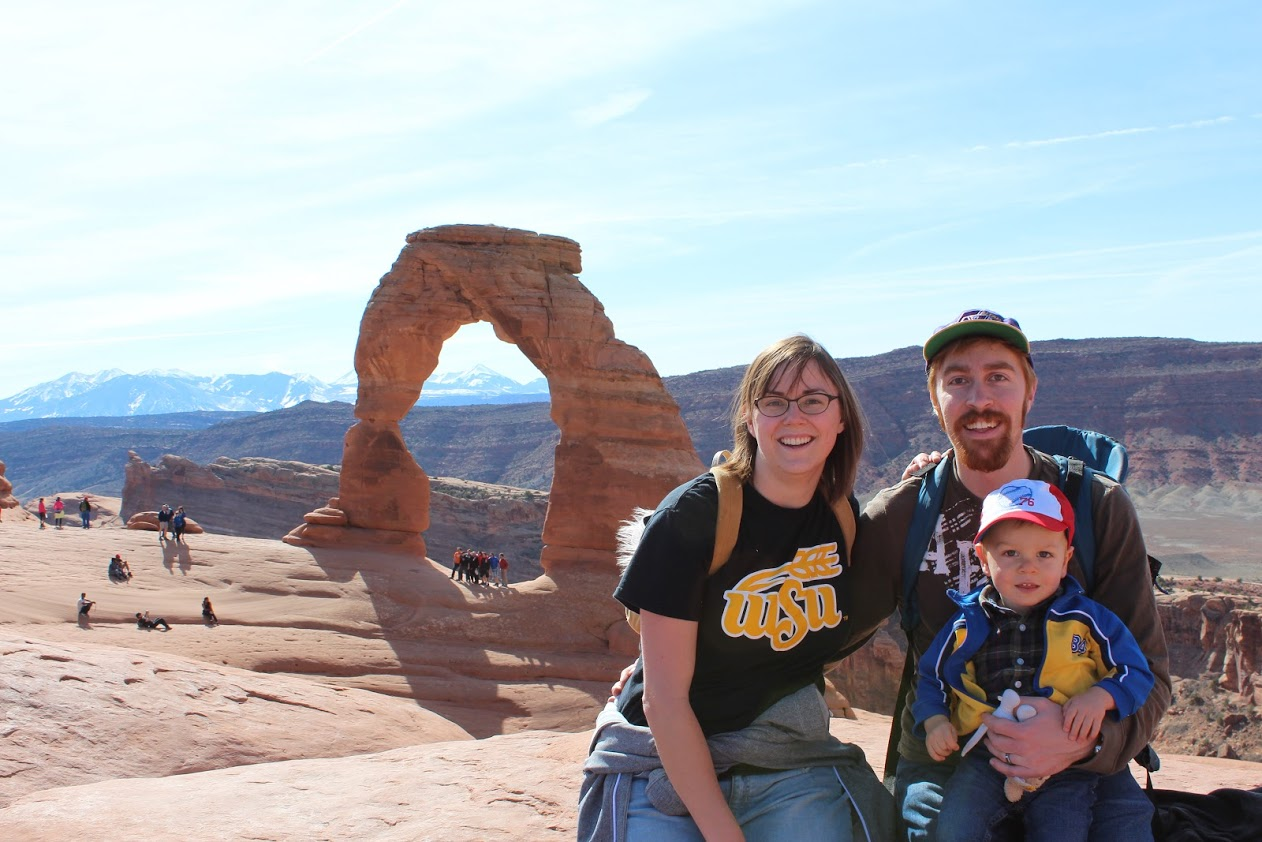
\includegraphics[width=0.7\linewidth]{../Figures/delicate_fam}
	\label{fig:delicate_fam}
	\end{figure}
\end{frame}

\begin{frame}
  \frametitle{outline}
  \setbeamertemplate{section in toc}[sections numbered]
  \tableofcontents[hideallsubsections]
\end{frame}

\section{fatigue}

\begin{frame}<handout:0>{intrinsic flaw}
	damage as function of tool speed
\end{frame}

\begin{frame}{fatigue}
	\begin{itemize}
		\item We refer to damage from repeated, or cyclic loads as fatigue damage
		\item Some of the earliest work on fatigue began in the 1800's
		\item Chains, railway axles, etc.
		\item An estimated 80\% of failure expenses are due to fatigue
	\end{itemize}
\end{frame}

\begin{frame}{fatigue}
	\begin{itemize}[<+->]
		\item There are three main approaches to fatigue analysis
		\item Stress based fatigue analysis
		\item Strain based fatigue analysis
		\item Fracture mechanics fatigue analysis
	\end{itemize}
\end{frame}

\begin{frame}{stress based fatigue}
	\begin{itemize}[<+->]
		\item One of the simplest assumptions we can make is that a load cycles between a constant maximum and minimum stress value
		\item This is a good approximation for many cases (axles, for example) and can also be easily replicated experimentally
		\item This is referred to as constant amplitude stressing
	\end{itemize}
\end{frame}

\begin{frame}{constant amplitude stressing}
	\begin{figure}
		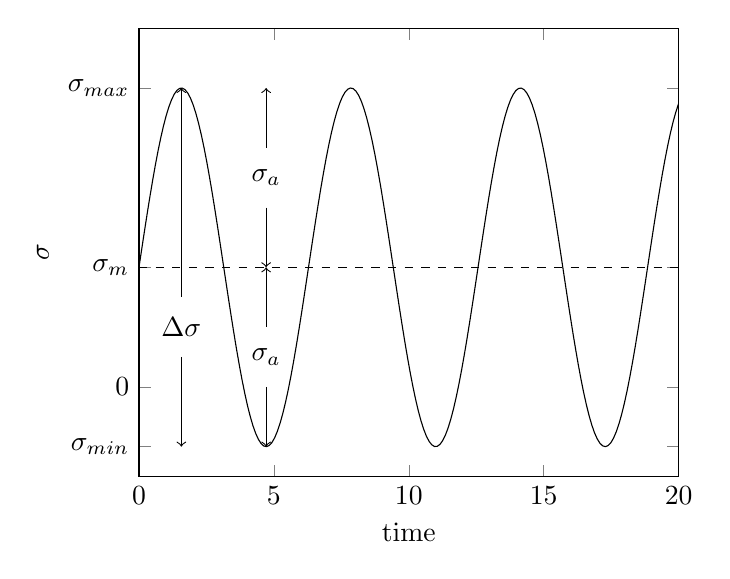
\begin{tikzpicture}
		\begin{axis}[
		domain=0:20,
		samples=200,
		xmin=0,   xmax=20,
		ymin=-3,   ymax=12,
		ylabel=$\sigma$,
		xlabel=time,
		ytick={-2, 0, 4, 10},
		yticklabels={$\sigma_{min}$, 0, $\sigma_m$, $\sigma_{max}$}]
		\addplot [color=black,mark=none] {6*sin(deg(x)) + 4};
		\addplot [color=black,style=dashed,mark=none] coordinates { (0,4) (20,4)};
		\draw[<-] (axis cs: 3.14159/2,10) -- (axis cs: 3.14159/2,3);
		\draw[->] (axis cs: 3.14159/2,1) -- (axis cs: 3.14159/2,-2);
		\draw node at (axis cs: 3.14159/2,2) {$\Delta \sigma$};
		\draw[<-] (axis cs: 3*3.14159/2,4) -- (axis cs: 3*3.14159/2,2);
		\draw[->] (axis cs: 3*3.14159/2,0) -- (axis cs: 3*3.14159/2,-2);
		\draw node at (axis cs: 3*3.14159/2,1) {$\sigma_a$};
		\draw[<-] (axis cs: 3*3.14159/2,10) -- (axis cs: 3*3.14159/2,8);
		\draw[->] (axis cs: 3*3.14159/2,6) -- (axis cs: 3*3.14159/2,4);
		\draw node at (axis cs: 3*3.14159/2,7) {$\sigma_a$};
		\end{axis}
		\end{tikzpicture}
	\end{figure}
\end{frame}

\begin{frame}{constant amplitude stressing}
	\begin{itemize}[<+->]
		\item $\Delta \sigma$ is known as the stress range, and is the difference between max and min stress
		\item $\sigma_m$ is the mean stress, and can sometimes be zero, but this is not always the case
		\item $\sigma_a$ is the stress amplitude, and is the variation about the mean
		\item We can express all of these in terms of the maximum and minimum stress
		\begin{align}
		\Delta \sigma &= \sigma_{max} - \sigma_{min}\\
		\sigma_m &= \frac{\sigma_{max} + \sigma_{min}}{2}\\
		\sigma_a &= \frac{\sigma_{max}- \sigma_{min}}{2}
		\end{align}
	\end{itemize}
\end{frame}

\begin{frame}{constant amplitude stressing}
	\begin{itemize}[<+->]
		\item It is also common to describe some ratios
		\item The stress ratio, $R$ is defined as
		\begin{equation}
		R = \frac{\sigma_{min}}{\sigma_{max}}
		\end{equation}
		\item And the amplitude ratio, $A$ is defined as
		\begin{equation}
		A = \frac{\sigma_a}{\sigma_m}
		\end{equation}
	\end{itemize}
\end{frame}

\begin{frame}{useful relations}
	\begin{itemize}
		\item There are some useful relationships between the above equations
		\begin{subequations}
			\begin{align}
			\Delta \sigma &= 2 \sigma_a = \sigma_{max}(1-R)\\
			\sigma_m &= \frac{\sigma_{max}}{2}(1+R)\\
			R &= \frac{1-A}{1+A}\\
			A &= \frac{1-R}{1+R}
			\end{align}
		\end{subequations}
	\end{itemize}
\end{frame}

\section{nominal and local stress}

\begin{frame}{definition and notation}
	\begin{itemize}[<+->]
		\item It is important to distinguish between the nominal (global) stress and the local stress at some point of interest
		\item We use $\sigma$ for the stress at a point (local stress)
		\item We use $S$ as the nominal (global) stress
		\item In simple tension, $\sigma = S$ 
		\item For many cases (bending, notches), $\sigma \ne S$ in general
		\item We must also be careful to note $\sigma_y$, in some cases $S < \sigma_y$ but at some locations $\sigma > \sigma_y$
	\end{itemize}
\end{frame}

\begin{frame}{simple tension}
	\begin{figure}
	\centering
	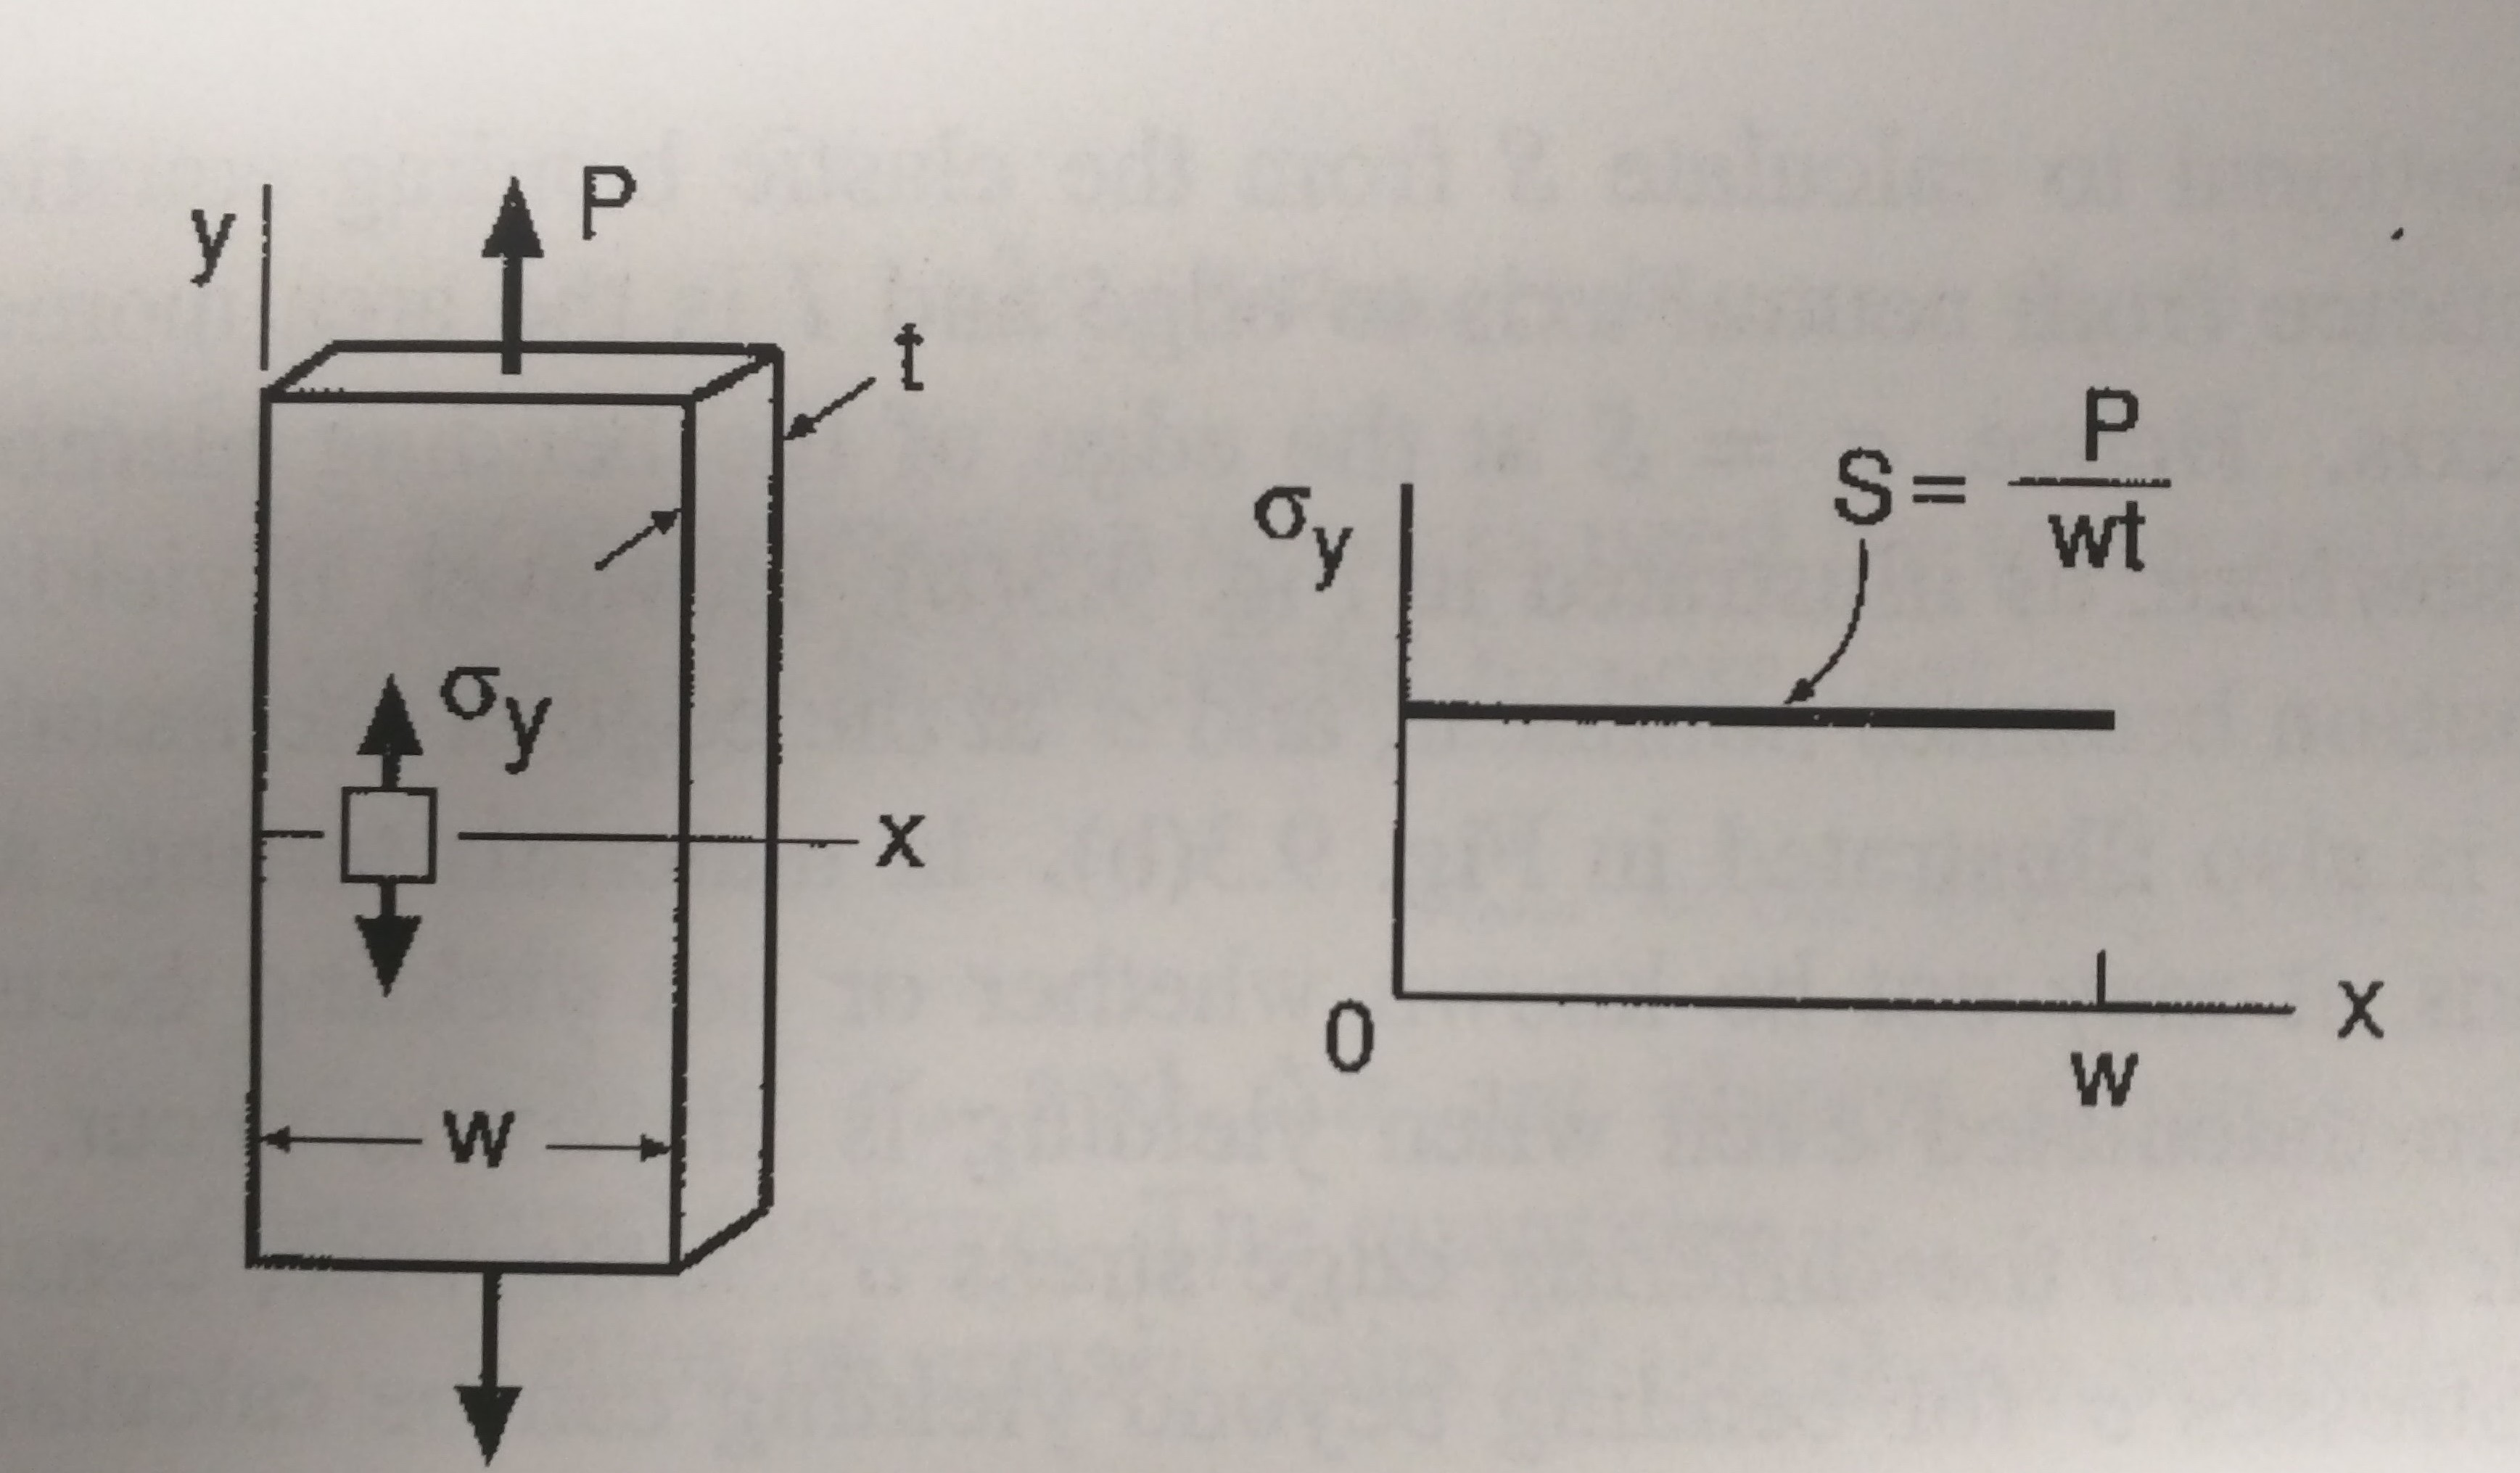
\includegraphics[width=0.7\linewidth]{../Figures/p232-a}
	\caption{In this case $S = \sigma$}
	\label{fig:p232-a}
	\end{figure}
\end{frame}

\begin{frame}{bending}
	\begin{figure}
	\centering
	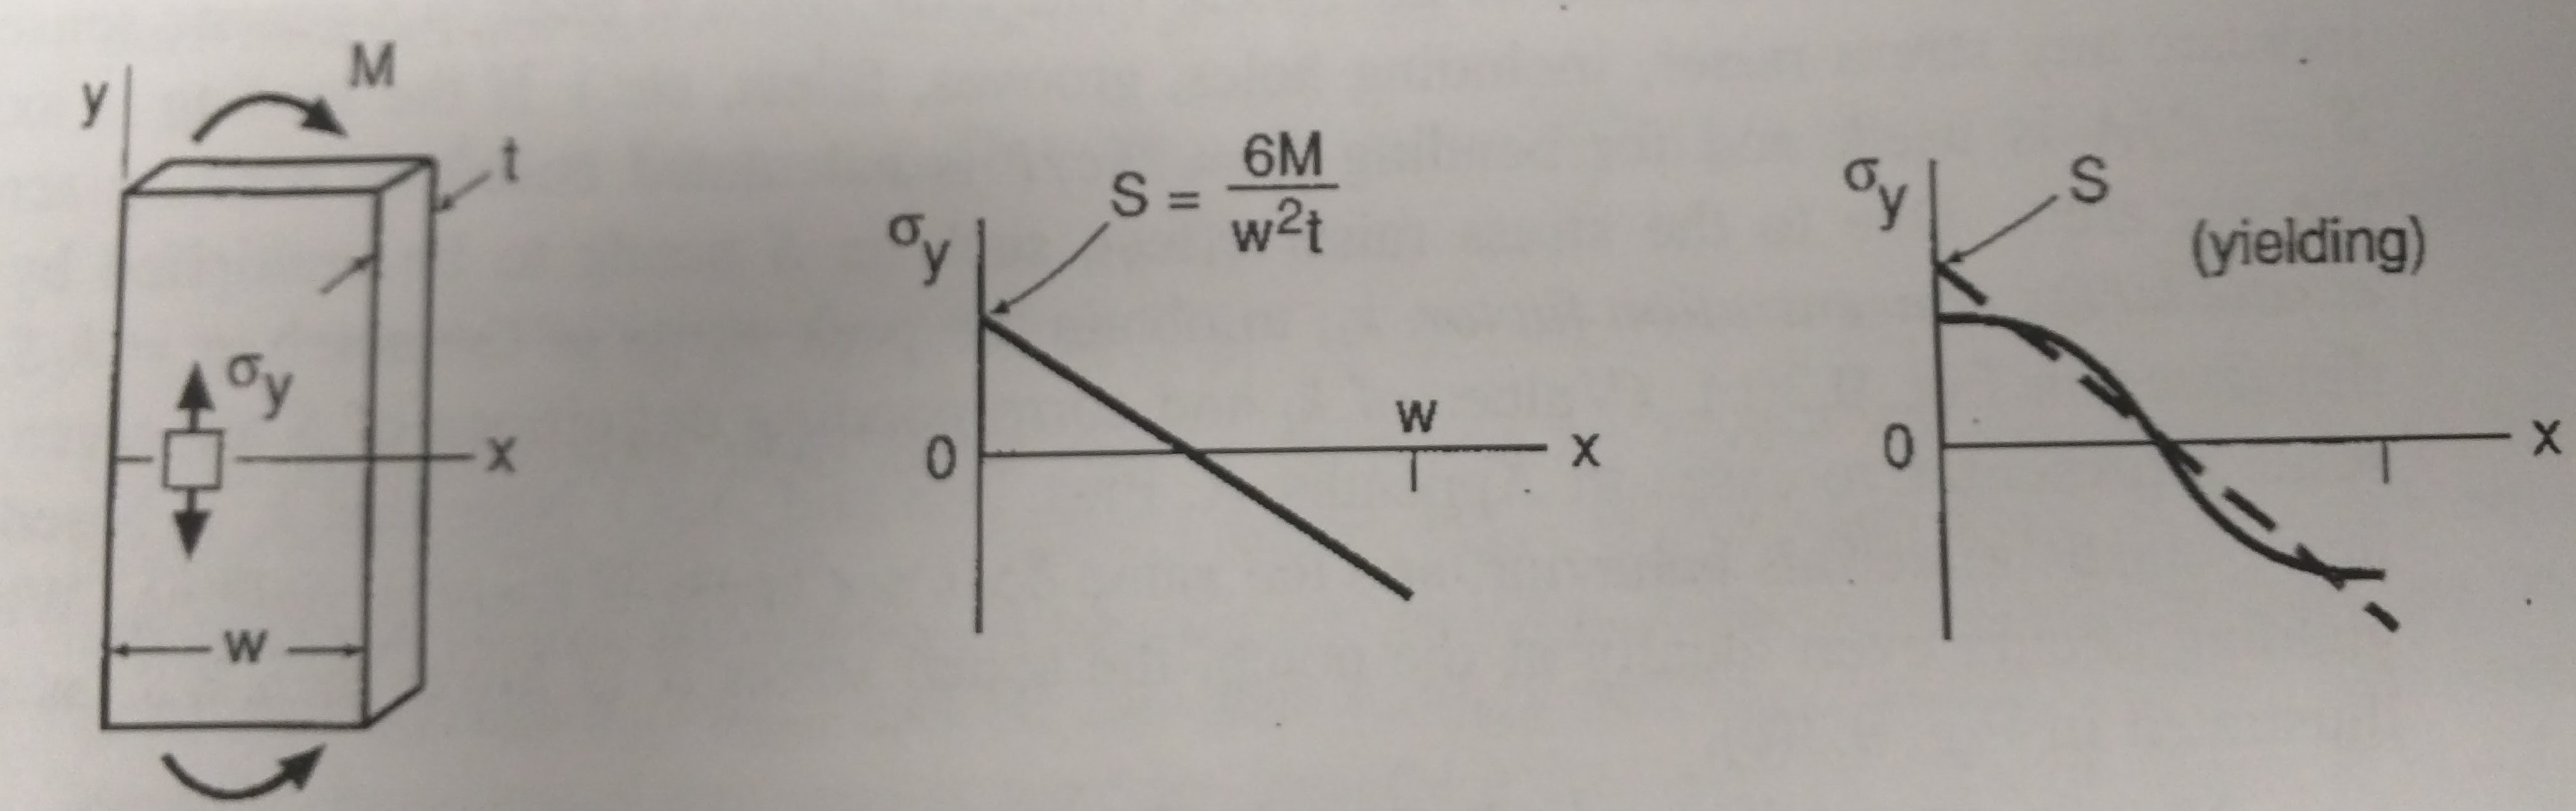
\includegraphics[width=0.7\linewidth]{../Figures/p232-b}
	\caption{As long as $\sigma < \sigma_y$, $\sigma$ varies linearly. If $\sigma > \sigma_y$ at any location, however, the relationship is non-linear}
	\label{fig:p232-b}
	\end{figure}
\end{frame}

\begin{frame}{notches}
	\begin{figure}
	\centering
	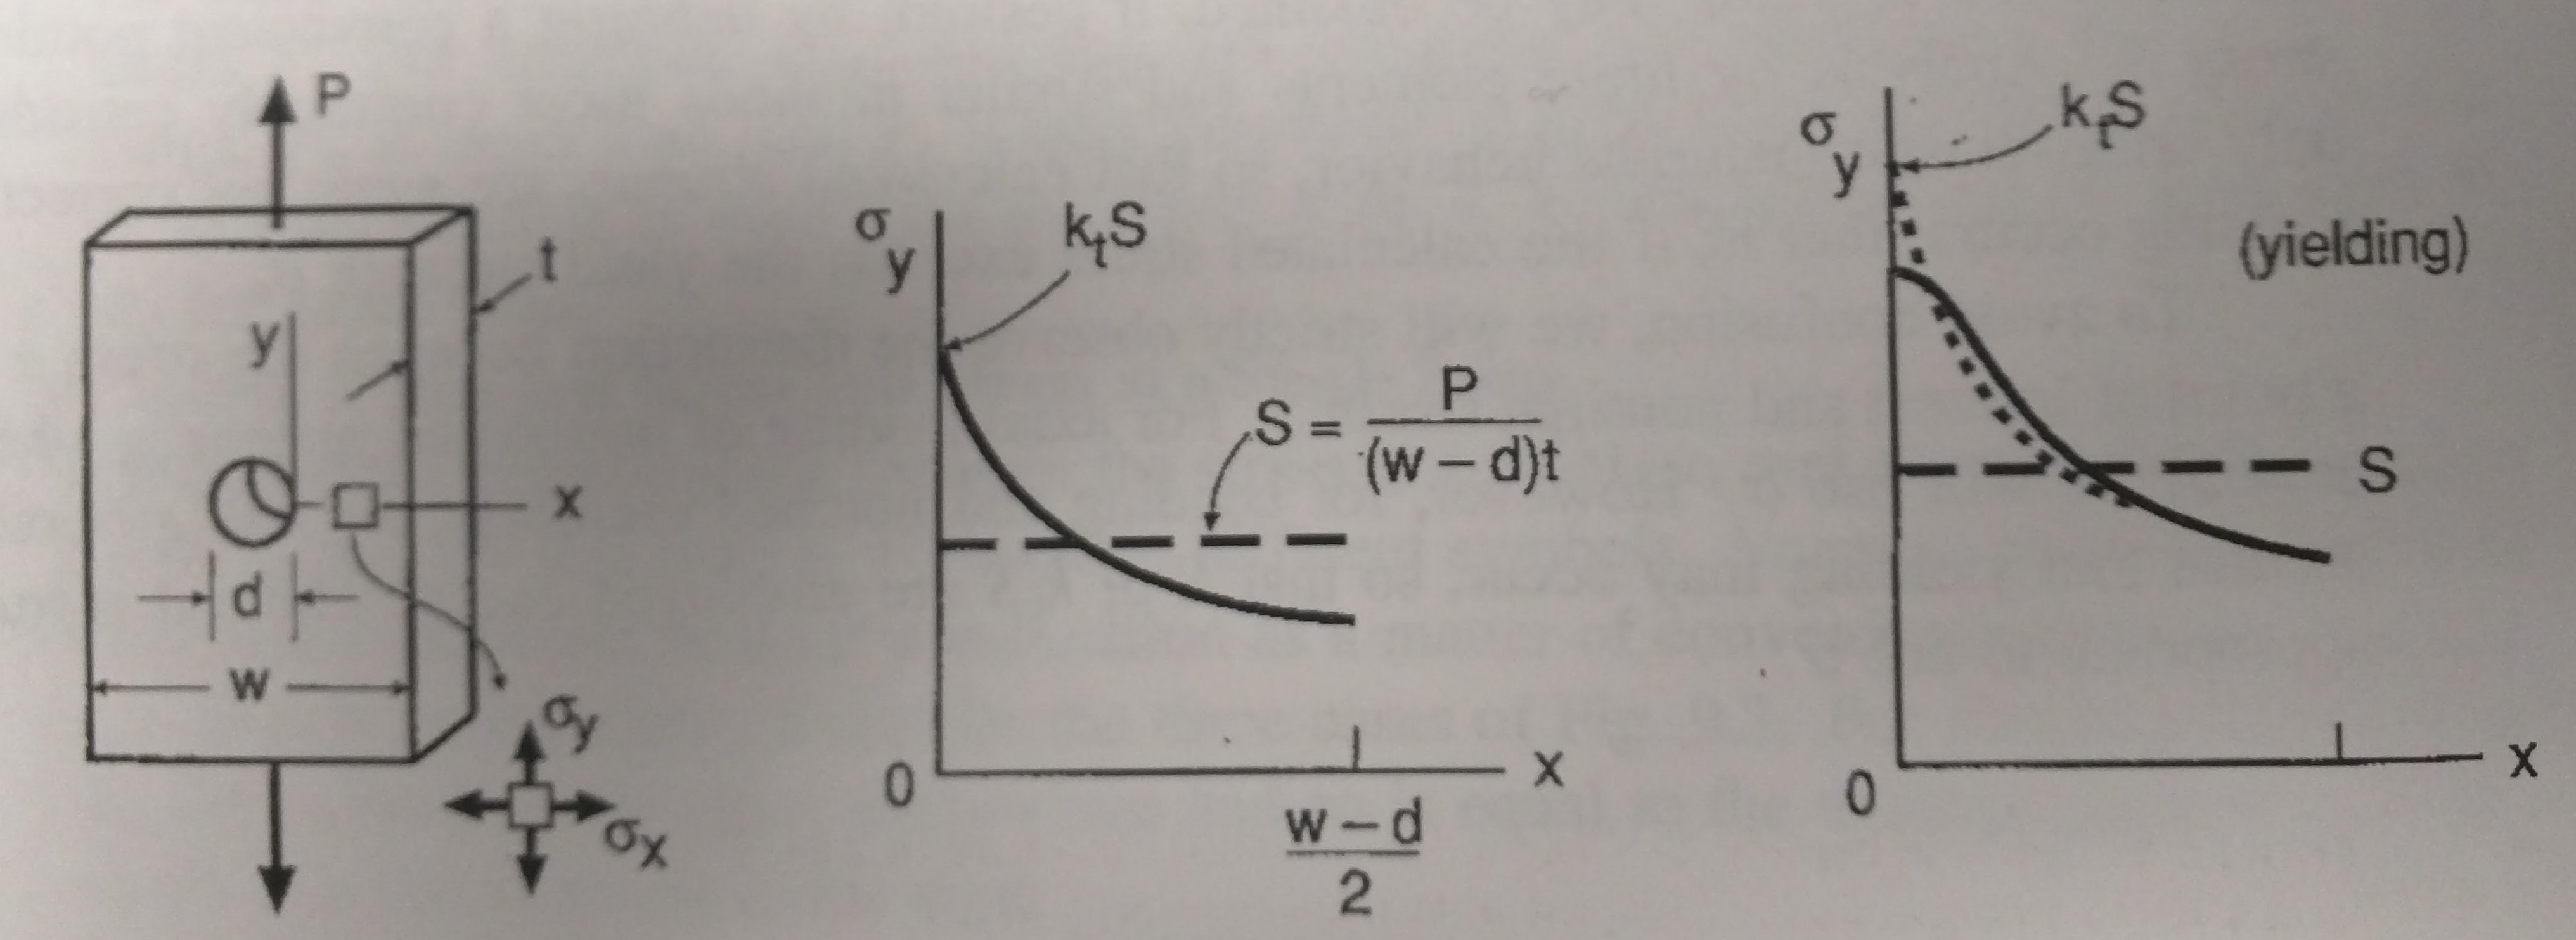
\includegraphics[width=0.7\linewidth]{../Figures/p232-c}
	\caption{As long as $\sigma < \sigma_y$, $\sigma$ varies linearly. If $\sigma > \sigma_y$ at any location, however, the relationship is non-linear}
	\label{fig:p232-c}
	\end{figure}
\end{frame}

\section{fatigue tests}

\begin{frame}{rotating cantilever beam}
	\begin{figure}
	\centering
	\includegraphics[width=0.7\linewidth]{"../Figures/rotating_cantilever"}
	\caption{Cantilever beam produces non-uniform stress state}
	\label{fig:rotatingcantilever}
	\end{figure}
\end{frame}

\begin{frame}{rotating four-point bend}
	\begin{figure}
	\centering
	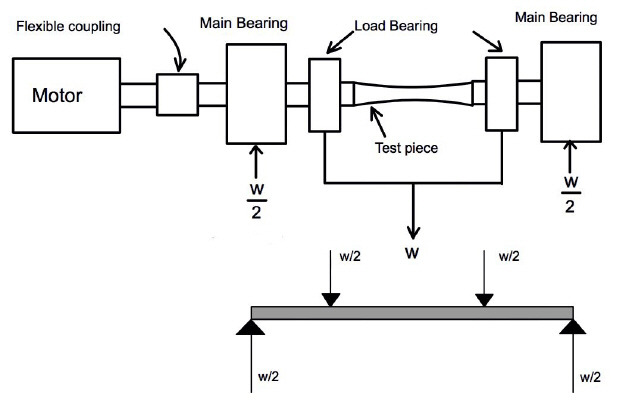
\includegraphics[width=0.7\linewidth]{../Figures/Rotating_Bending_Machine}
	\caption{Four-point bend gives uniform stress (along top and bottom surfaces)}
	\label{fig:Rotating_Bending_Machine}
	\end{figure}
\end{frame}

\begin{frame}{fatigue tests}
	\begin{itemize}[<+->]
		\item The above rotating methods are very common, but in their current configurations can only be used for zero mean stress
		\item a reciprocating bend test can be used for non-zero mean stress
	\end{itemize}
\end{frame}

\begin{frame}{reciprocating bend test}
	\begin{figure}
	\centering
	\includegraphics[width=0.7\linewidth]{"../Figures/reciprocating_cantilever"}
	\caption{A reciprocating cantilever test allows for non-zero mean stress}
	\label{fig:reciprocatingcantilever}
\end{figure}
\end{frame}

\begin{frame}{axial fatigue test}
	\begin{figure}
	\centering
	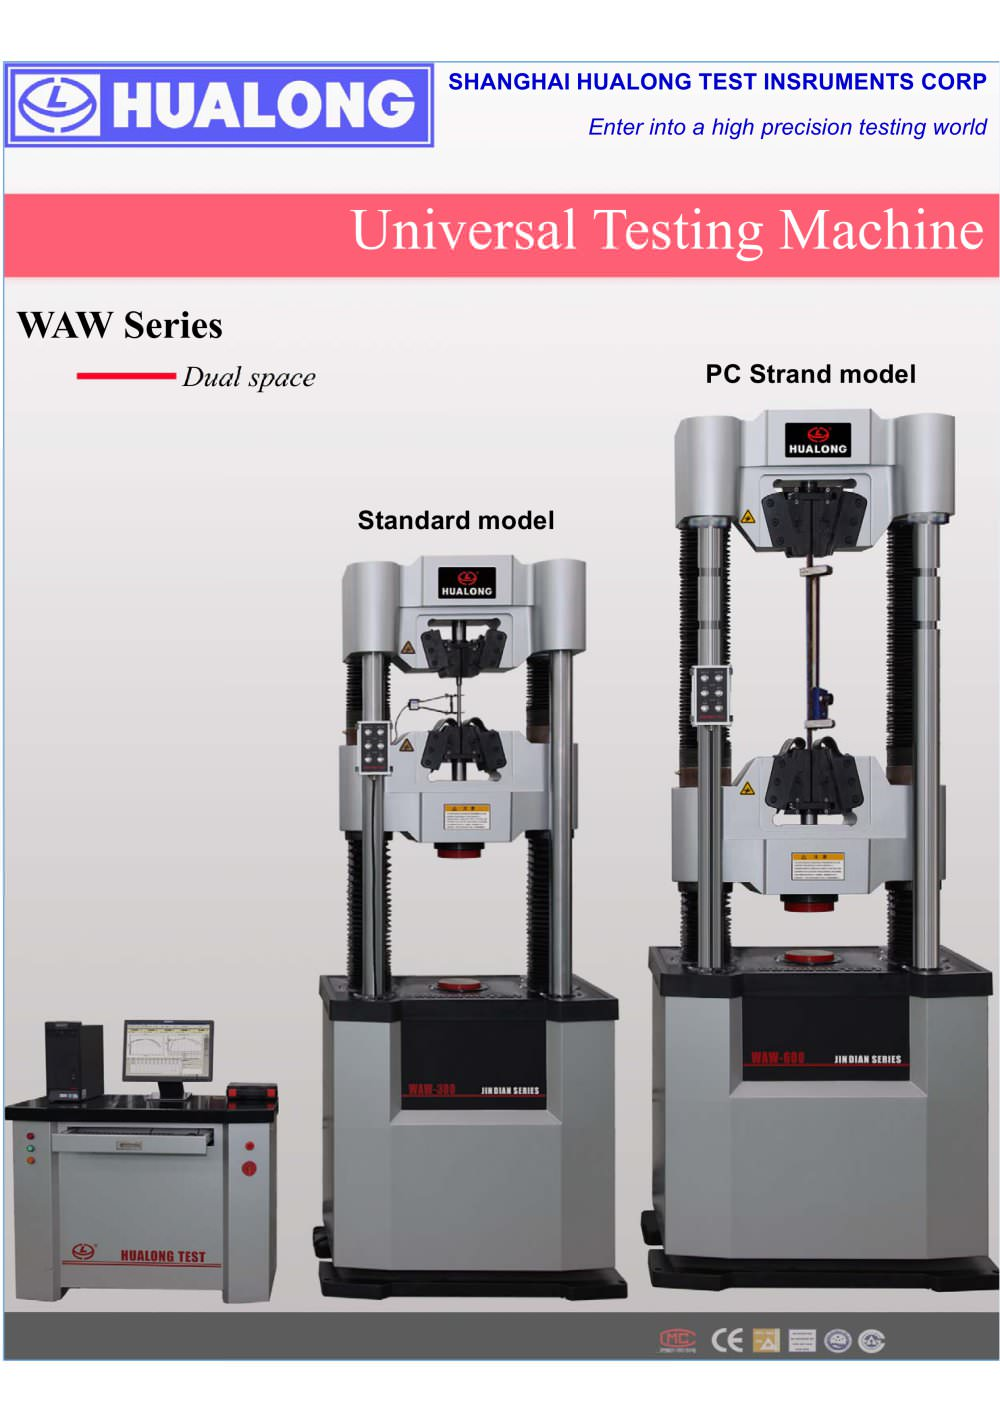
\includegraphics[width=0.7\linewidth]{../Figures/servohydraulic}
	\caption{Servohydraulic test fixtures are expensive, but computer controlled and allow for irregular load histories}
	\label{fig:servohydraulic}
	\end{figure}
\end{frame}

\begin{frame}{fatigue tests}
	\begin{itemize}[<+->]
		\item The length of a fatigue test is determined by two factors
		\begin{enumerate}
			\item How many cycles it takes for the specified load to cause failure
			\item The speed of the motor controlling the test
		\end{enumerate}
		\item Servohydraulic machines generally have a speed of 10 - 100 Hz.
		\item At a speed of 100 Hz, it would take 28 hours for $10^7$ cycles, 12 days for $10^8$ cycles, and nearly 4 months for $10^9$ cycles
		\item While some machines can test at very high speeds, the inertia of the sample can interfere with results
	\end{itemize}
\end{frame}

\section{fatigue life analysis}

\begin{frame}{stress life curves}
	\begin{itemize}[<+->]
		\item Stress-life curves, or S-N curves, are generated from test data to predict the number of cycles to failure
		\item In general, one set (or family) of S-N curves is generated using the same $\sigma_m$
		\item Usually $S_a$ (the nominal stress equivalent of $\sigma_a$) is plotted versus $N$ (the number of cycles)
	\end{itemize}
\end{frame}

\begin{frame}{stress life curves}
	\begin{itemize}[<+->]
		\item Each individual point on an S-N curve represents one fatigue experiment
		\item To find enough data to form statistical significance, as well as to fit a curve across all levels of fatigue is very time-consuming
		\item In the following plot, if only one test was performed for each point, the total number of cycles tested would be about $7.3x10^7$
		\item For a 100 Hz machine, this represents over 200 hours of consecutive testing
		\item Each repetition would further increase the test time required
	\end{itemize}
\end{frame}

\begin{frame}{stress life curves}
	\begin{tikzpicture}
	\begin{axis}[%
		xlabel={$N_f$ (cycles to failure)},%
		ylabel={$S_a$ (MPa)}]
	\addplot[only marks] coordinates {
		(50043.42952596336,304.3384885916487)
		(61810.2778157969,275.4565502529583)
		(64649.06882505588,262.997448795745)
		(169586.85224960672,247.7449948831778)
		(565161.8625105635,233.04313985499925)
		(761338.8628672551,220.14010003026843)
		(1579862.092639026,191.8692976260827)
		(3173264.1073141545,178.55402931722847)
		(3682937.77739026,205.51896106891124)
		(9552328.626265539,185.27652459677992)
		(18242638.367873847,164.96778564118816)
		(35011737.76351732,165.60774874241474)
		};
	\end{axis}
	\end{tikzpicture}
\end{frame}

\begin{frame}{stress life curves}
	\begin{itemize}[<+->]
		\item On a linear scale, the data appear not to agree well with any standard fit
		\item It is also very difficult to differentiate between low-cycle fatigue failure stresses
		\item Instead S-N curves are often plotted on a semi-log or log-log scale, so pay attention to the axes
	\end{itemize}
\end{frame}

\begin{frame}{stress life curves}
	\begin{tikzpicture}
	\begin{axis}[%
	xmode=log,%
	xlabel={$N_f$ (cycles to failure)},%
	ylabel={$S_a$ (MPa)}]
	\addplot[only marks] coordinates {
		(50043.42952596336,304.3384885916487)
		(61810.2778157969,275.4565502529583)
		(64649.06882505588,262.997448795745)
		(169586.85224960672,247.7449948831778)
		(565161.8625105635,233.04313985499925)
		(761338.8628672551,220.14010003026843)
		(1579862.092639026,191.8692976260827)
		(3173264.1073141545,178.55402931722847)
		(3682937.77739026,205.51896106891124)
		(9552328.626265539,185.27652459677992)
		(18242638.367873847,164.96778564118816)
		(35011737.76351732,165.60774874241474)
	};
	\end{axis}
	\end{tikzpicture}
\end{frame}

\begin{frame}{curve fits}
	\begin{itemize}[<+->]
		\item If the curve is nearly linear on a log-linear plot, we use the following form to fit the data
		\item \begin{equation}
		\sigma_a = C + D \log N_f
		\end{equation}
		\item When the data are instead linear on a log-log scale, the following form is generally used
		\item \begin{equation}
		\sigma_a = \sigma_f^\prime \left(2N_f\right)^b
		\end{equation}
		\item $\sigma_f^\prime$ and $b$ are often considered material properties and can often be looked up on a table (p. 235)
	\end{itemize}
\end{frame}

\begin{frame}{curve fit}
	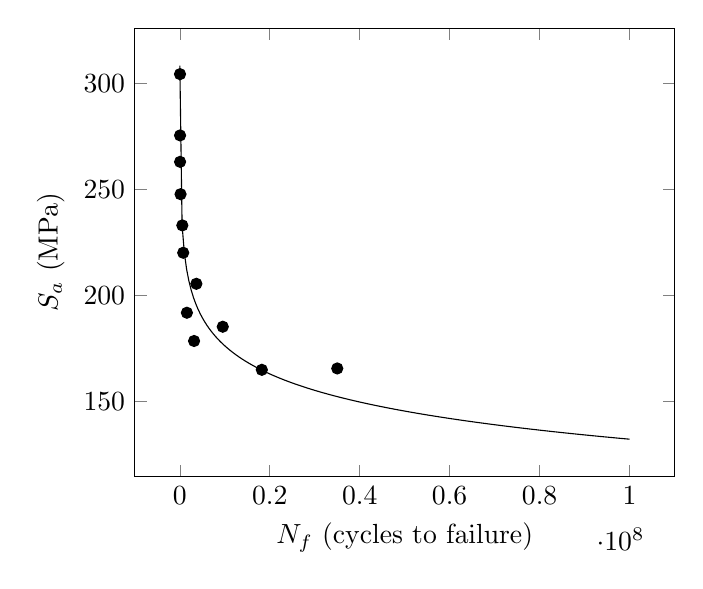
\begin{tikzpicture}
	\begin{axis}[%
	domain=1e4:1e8,%
	samples=200,%
	xlabel={$N_f$ (cycles to failure)},%
	ylabel={$S_a$ (MPa)}]
	\addplot[only marks] coordinates {
		(50043.42952596336,304.3384885916487)
		(61810.2778157969,275.4565502529583)
		(64649.06882505588,262.997448795745)
		(169586.85224960672,247.7449948831778)
		(565161.8625105635,233.04313985499925)
		(761338.8628672551,220.14010003026843)
		(1579862.092639026,191.8692976260827)
		(3173264.1073141545,178.55402931722847)
		(3682937.77739026,205.51896106891124)
		(9552328.626265539,185.27652459677992)
		(18242638.367873847,164.96778564118816)
		(35011737.76351732,165.60774874241474)
	};
	\addplot[no markers] {484.47 - 19.12*ln(x)};
	\end{axis}
	\end{tikzpicture}
\end{frame}

\begin{frame}{stress life curves}
	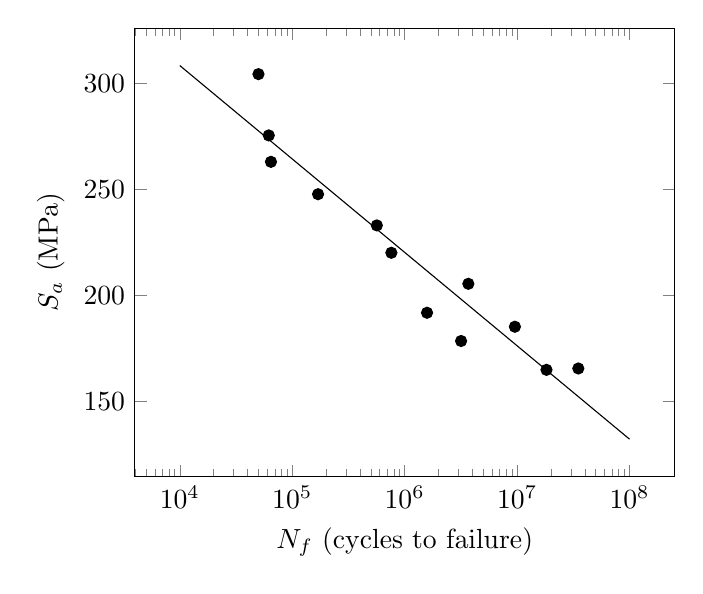
\begin{tikzpicture}
	\begin{axis}[%
	xmode=log,%
	domain=1e4:1e8,%
	samples=200,%
	xlabel={$N_f$ (cycles to failure)},%
	ylabel={$S_a$ (MPa)}]
	\addplot[only marks] coordinates {
		(50043.42952596336,304.3384885916487)
		(61810.2778157969,275.4565502529583)
		(64649.06882505588,262.997448795745)
		(169586.85224960672,247.7449948831778)
		(565161.8625105635,233.04313985499925)
		(761338.8628672551,220.14010003026843)
		(1579862.092639026,191.8692976260827)
		(3173264.1073141545,178.55402931722847)
		(3682937.77739026,205.51896106891124)
		(9552328.626265539,185.27652459677992)
		(18242638.367873847,164.96778564118816)
		(35011737.76351732,165.60774874241474)
	};
	\addplot[no markers] {484.47 - 19.12*ln(x)};
	\end{axis}
	\end{tikzpicture}
\end{frame}

\section{fatigue limit}

\begin{frame}{fatigue limit}
	\begin{itemize}[<+->]
		\item The fatigue limit, or endurance limit, is a feature of some materials where below a certain stress, no fatigue failure is observed
		\item Below the fatigue limit, this material is considered to have infinite life
		\item This most notably occurs in plain-carbon and low-alloy steels
		\item In these materials, $\sigma_e$ is considered to be a material property
		\item This phenomenon is not typical of aluminum or copper alloys, but is sometimes arbitrarily assigned using whatever the failure stress is at some large number of cycles ($10^7$ or $10^8$)
	\end{itemize}
\end{frame}

\begin{frame}{fatigue limit}
	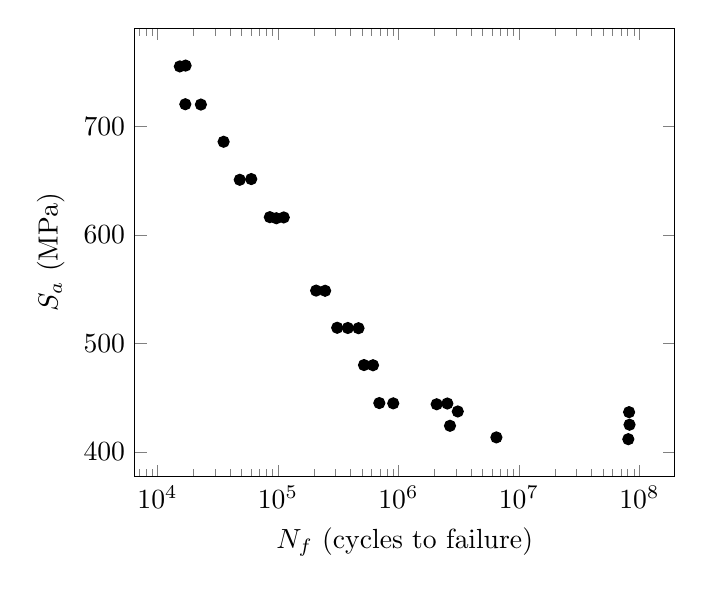
\begin{tikzpicture}
	\begin{axis}[%
	xmode=log,%
	domain=1e3:1e8,%
	samples=200,%
	xlabel={$N_f$ (cycles to failure)},%
	ylabel={$S_a$ (MPa)}]
	\addplot[only marks] coordinates {
		(15335.57305076729,755.3980800096908)
		(17120.563873524803,756.1781896368977)
		(17030.666340686137,720.548741709821)
		(22930.156230029723,720.2495381726781)
		(35394.72596452449,685.9598437358045)
		(48178.50680065504,650.9057872263105)
		(60015.34650935311,651.5756639714122)
		(85619.60323966984,616.4743647981587)
		(96991.95509887673,615.4580418521547)
		(111725.20919888247,616.2066563701887)
		(310167.4766824342,514.5113715514369)
		(380171.36929461616,514.3066533418128)
		(465974.9357903219,514.1019351321886)
		(207329.98874026354,548.7695708791375)
		(246290.6168802425,548.5963477786863)
		(517751.44153305655,480.1429393416311)
		(615045.2363433094,479.96971624117987)
		(693804.9505813519,445.1046303867236)
		(905347.6109897072,444.8369219587535)
		(2075614.3484015197,444.00230156567034)
		(2545405.291185992,444.68792586535835)
		(3106869.8968525752,437.3604675812362)
		(2677489.704626086,424.14705793283065)
		(6497638.107517564,413.4556797189666)
		(82022604.86227266,436.74025620059956)
		(82752208.82434484,425.1500560249538)
		(80830258.5708036,411.81066593985645)
	};
	\end{axis}
	\end{tikzpicture}
\end{frame}

\begin{frame}{high and low cycle fatigue}
	\begin{itemize}[<+->]
		\item Some other important terms are high cycle fatigue and low cycle fatigue
		\item "High cycle fatigue" generally is considered anything above $10^3$ cycles, but varies somewhat by material
		\item High cycle fatigue occurs when the stress is sufficiently low that yielding effects do not dominate behavior
		\item When yielding effects do dominate behavior, the strain-based approach is more appropriate
	\end{itemize}
\end{frame}
\end{document}
